\documentclass[referee,lineno,pdflatex]{sn-jnl}

\usepackage{float}

\usepackage{bookmark}
\usepackage{graphicx}
\usepackage{multirow}
\usepackage{amsmath,amssymb,amsfonts}
\usepackage[title]{appendix}
\usepackage{xcolor}
\usepackage{textcomp}
\usepackage{manyfoot}
\usepackage{booktabs}
\usepackage{array}
\usepackage{tabularx}

\raggedbottom
\articletype{Research}

\begin{document}

\title[Evidence-guided LLM refinement]{DeepSeekCell: evidence-guided selective refinement for large language model annotation of single-cell RNA-seq}

\author[1]{\fnm{Mohamed} \sur{Kone}}
\author*[1]{\fnm{Shulin} \sur{Wang}}\email{books@hnu.edu.cn}
\author[1]{\fnm{Gaoussou} \sur{Haidara}}

\affil*[1]{\orgname{School of Computer Science and Engineering, Hunan University}, \orgaddress{\city{Changsha}, \country{China}}}

\abstract{\textbf{Background:} Accurate cell type annotation remains a critical step in single-cell RNA sequencing (scRNA-seq) analysis. Large language models (LLMs) can interpret marker genes using broad biomedical knowledge, but unconstrained LLM annotation can be difficult to audit, weakly linked to controlled vocabularies, and inefficient if every uncertain cluster receives repeated model inference. A central methodological question is whether deterministic biological evidence can identify the subset of clusters that most deserves a second LLM pass.

\textbf{Results:} We developed DeepSeekCell, an evidence-guided LLM framework for marker-based scRNA-seq cell type annotation. DeepSeekCell performs structured first-pass annotation from cluster marker genes, maps labels to the Cell Ontology, scores deterministic evidence from ontology support, marker-profile agreement, tissue consistency, and mixed-cluster signals, and selectively invokes a second LLM pass only for clusters with discordant biological evidence. The framework also provides evidence-adjusted confidence scores, ranked candidate cell types, provenance fields, and an interactive Shiny implementation supporting DeepSeek API and local Ollama models.

Benchmarking was performed under a marker-driven cluster annotation scenario across six publicly available scRNA-seq datasets representing immune, pancreatic, brain, and lung tissues. A paired ablation design reused the same cached first-pass LLM response across all DeepSeekCell arms, separating first-pass prompting, evidence scoring, confidence adjustment, and second-pass refinement. DeepSeekCell-SelfRefined increased mean macro-F1 from 0.733 for the first-pass LLM to 0.794 and mean ontology-aware clade accuracy from 0.883 to 0.893. The strongest result was refinement efficiency: evidence-guided selective refinement recovered 59.1\% of all corrections achieved by full refinement while refining only 6.4\% as many clusters, corresponding to a correction efficiency of 81.3\%, compared with 56.3\% for random selection, 43.8\% for confidence-based selection, and 8.8\% for full refinement. No refinement strategy introduced incorrect revisions of previously correct annotations. Native cell-level CellTypist, SingleR, ScType, and scmap baselines were included for external comparison.

\textbf{Conclusions:} DeepSeekCell reframes LLM-based cell type annotation as an evidence allocation problem: deterministic marker and ontology evidence can identify the clusters where additional LLM reasoning is most useful. This selective refinement strategy provides an auditable and cost-aware path for explainable single-cell annotation beyond a simple LLM wrapper.}

\keywords{single-cell RNA sequencing, cell type annotation, large language models, selective refinement, confidence calibration, Cell Ontology, explainable artificial intelligence, DeepSeek, bioinformatics}

\maketitle

\section{Introduction}\label{sec:introduction}

Single-cell RNA sequencing (scRNA-seq) enables high-resolution analysis of cellular heterogeneity across tissues, development, and disease. A central interpretive step in scRNA-seq analysis is assigning biological identities to transcriptionally defined clusters or individual cells. In practice, this process often relies on expert interpretation of marker genes, comparison with reference atlases, and iterative inspection of tissue context. Manual annotation is powerful, but it can be subjective, labor-intensive, and difficult to reproduce across laboratories.

Automated annotation methods have improved scalability. Reference-based approaches such as SingleR and scmap compare query profiles with labeled references or projected cell states \cite{aran2019singler,singlerbook,kiselev2018scmap}. Marker- and model-guided approaches such as ScType, CellAssign, Garnett, and CellTypist use curated marker combinations, probabilistic assignment, supervised classification, or pretrained cell type models to identify cell identities \cite{ianevski2022sctype,zhang2019cellassign,pliner2019garnett,dominguezconde2022celltypist}. These methods are widely useful, but each depends on the quality, coverage, and specificity of reference data, marker databases, or training labels. They can also return labels that differ in granularity, terminology, or ontology compatibility, making downstream comparison across datasets difficult.

Large language models (LLMs) offer a complementary strategy because they can reason over marker gene lists and tissue context using broad biomedical knowledge. Direct applications to scRNA-seq annotation include GPTCelltype, which evaluated GPT-4 for marker-based cell type assignment \cite{hou2024gpt4}, scExtract for automated annotation and prior-informed integration \cite{wu2025scextract}, CASSIA for multi-agent interpretable annotation \cite{xie2025cassia}, mLLMCelltype for multi-model consensus annotation \cite{yang2026mllmcelltype}, LICT for reliability assessment \cite{ye2025lict}, AnnDictionary for benchmarking LLM behavior across cell and gene-set tasks \cite{crowley2025anndictionary}, and DeepCellSeek for large-scale benchmarking of multiple LLM families in cell typing \cite{xiao2025deepcellseek}. In parallel, single-cell foundation and language-inspired models such as scBERT, Geneformer, scGPT, and scFoundation have shown the value of large-scale transcriptomic pretraining for cell representation, network biology, and downstream annotation tasks \cite{yang2022scbert,theodoris2023geneformer,cui2024scgpt,hao2024scfoundation}.

Broader biomedical and omics-oriented LLM work further motivates this direction. Domain-adapted biomedical LLMs such as BioGPT and Med-PaLM illustrate the value and limitations of specializing language models for biomedical literature, question answering, and reasoning \cite{luo2022biogpt,singhal2023medpalm}. Tool-augmented approaches such as GeneGPT show that LLMs can be connected to external biomedical resources \cite{jin2024genegpt}, while recent gene-set interpretation systems demonstrate that LLMs can synthesize functional hypotheses from omics-derived gene groups but require safeguards against hallucination and unsupported claims \cite{hu2025genesetllm,wang2025geneagent}. However, free-text LLM annotation introduces new challenges: outputs may be inconsistent across runs, difficult to validate automatically, weakly linked to controlled vocabularies, and insufficiently transparent for publication-grade analysis. For scRNA-seq annotation, an LLM-based system should therefore constrain outputs, expose reasoning, map labels to formal ontologies, and provide reproducible exports.

Despite rapid progress, there remains a need for annotation systems that combine biological knowledge-driven prediction, formal ontology integration, explainability, and efficient allocation of expensive LLM reasoning. DeepSeekCell was designed to address this gap. The framework combines marker-guided LLM annotation with Cell Ontology normalization \cite{cellontology,tan2025cellontology}, deterministic evidence scoring, confidence adjustment, selective self-refinement, and an interactive Shiny interface \cite{shiny}. Its main contributions are: (i) structured LLM-based annotation from cluster marker genes, (ii) tissue-aware Cell Ontology mapping with match provenance, (iii) deterministic marker, ontology, and tissue-consistency evidence scoring, (iv) evidence-adjusted confidence estimation and conflict detection, (v) selective second-pass refinement under compute-matched random and confidence-based controls, and (vi) a reproducible benchmark comparing the method with SingleR, ScType, scmap, and native CellTypist baselines across immune, pancreatic, brain, and lung datasets. The Shiny application serves as the dissemination layer for this evidence-guided annotation method.

\section{Methods}\label{sec:methods}

\subsection{Overall framework}

DeepSeekCell is implemented as an R package with an interactive Shiny application. The overall workflow is: input marker genes, prompt engineering, first-pass DeepSeek or Ollama annotation, structured JSON parsing, Cell Ontology mapping, deterministic evidence scoring, evidence-adjusted confidence estimation, selective refinement of conflicted clusters, validation, visualization, and export. The package provides functions for marker preprocessing, prompt construction, LLM API access, response parsing, Cell Ontology mapping, evidence scoring, refinement prompting, report generation, and benchmarking. The Shiny application provides a browser-based workflow for entering marker genes, selecting model and metadata options, running annotation, inspecting results, viewing confidence summaries, reviewing explainability fields, and exporting reports. The workflow is shown in Fig.~\ref{fig:workflow}.

\begin{figure}[htp]
\centering
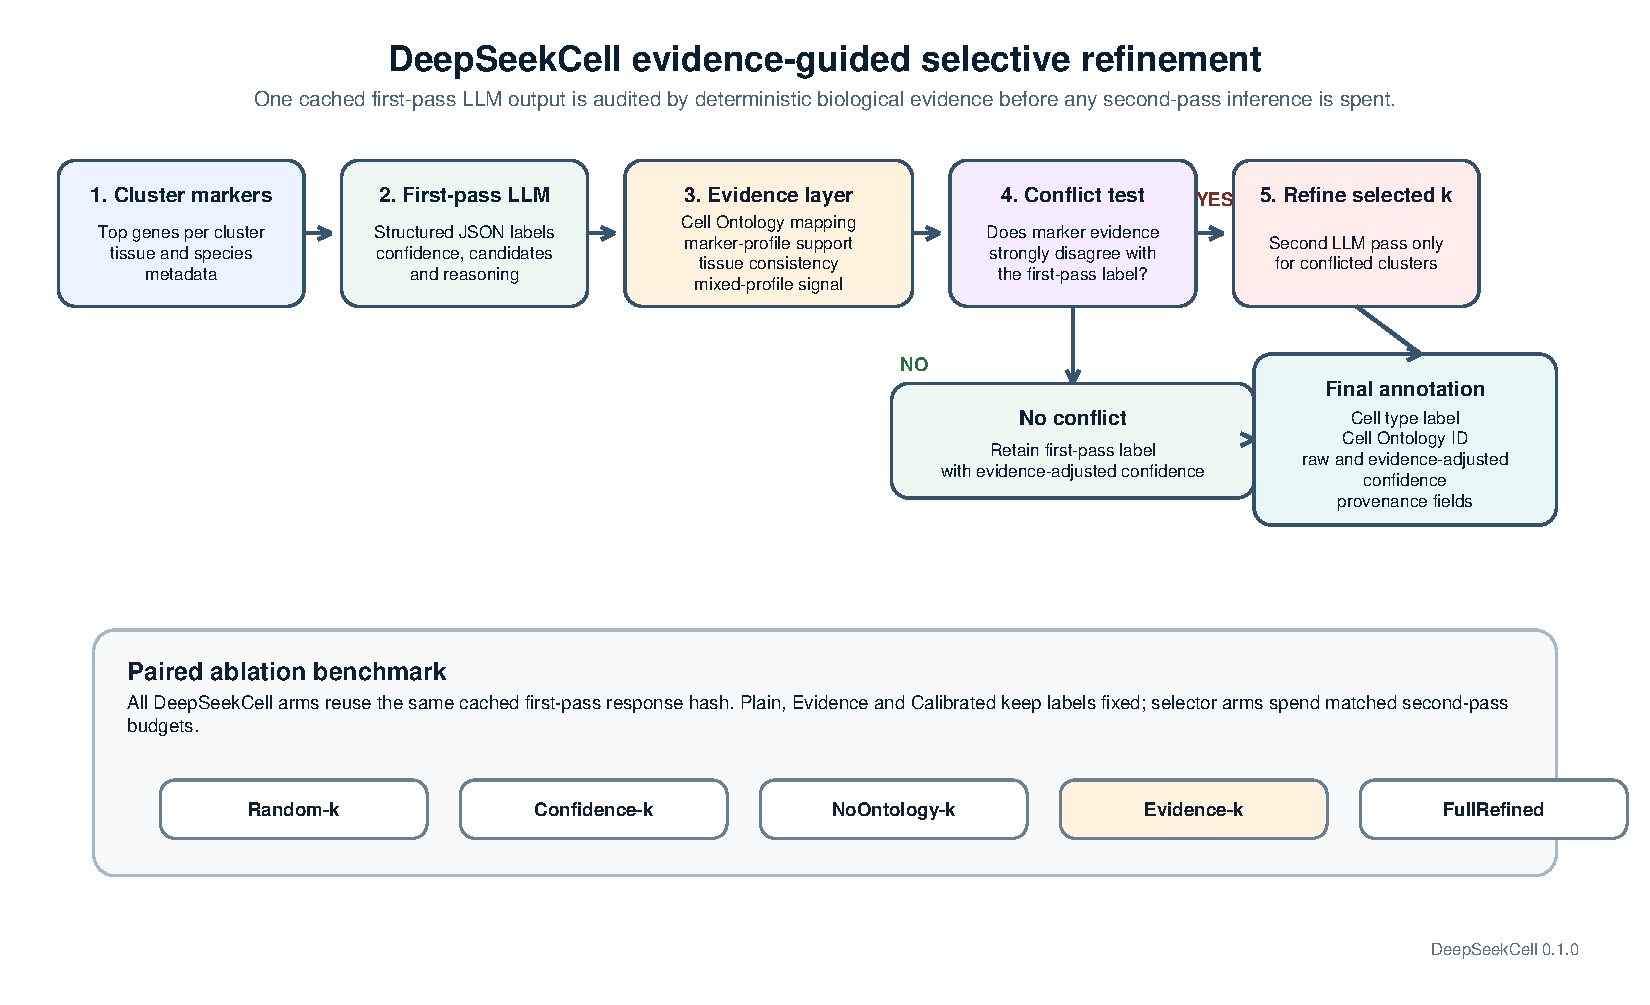
\includegraphics[width=\textwidth]{deepseekcell_workflow.pdf}
\caption{DeepSeekCell workflow. Cluster marker genes, tissue, and species metadata are submitted through the R API or Shiny interface. The framework applies marker processing and prompt engineering, sends a structured prompt to the selected DeepSeek or Ollama backend, parses the JSON response, maps the annotation to the Cell Ontology, evaluates deterministic biological evidence, flags conflicted clusters for selective refinement, visualizes confidence and ontology metadata, and exports tabular or HTML reports with marker-based reasoning.}\label{fig:workflow}
\end{figure}

The current software version is 0.1.0. OpenAI/GPT-4o support was removed from the maintained application surface to keep the publication version focused, reproducible, and aligned with the DeepSeekCell naming and benchmark design. The main software features of the publication release are summarized in Table~\ref{tab:features}.

\begin{table}[htp]
\caption{Main DeepSeekCell software features.}\label{tab:features}
\begin{tabular}{@{}ll@{}}
\toprule
Feature & DeepSeekCell support\\
\midrule
Marker-guided annotation & Yes\\
Interactive Shiny interface & Yes\\
Cell Ontology ID mapping & Yes\\
Ontology match provenance & Exact, synonym, context exact, fuzzy\\
Explainable marker reasoning & Yes\\
Confidence score & Yes\\
Tissue consistency flag & Yes\\
Mixed-cluster flag & Yes\\
CSV, XLSX, and HTML export & Yes\\
Benchmark scripts & Yes\\
Offline fallback ontology & Yes\\
\botrule
\end{tabular}
\end{table}

\subsection{Marker gene processing}

DeepSeekCell accepts per-cluster marker genes as comma-, semicolon-, whitespace-, or newline-separated text. Marker processing standardizes gene symbols, removes duplicates, filters common low-information genes, including mitochondrial, ribosomal, and pseudogene-like features, and preserves the top marker genes selected from upstream clustering analysis. The benchmark workflow used the top 25 marker genes per cluster. The Shiny interface currently accepts marker genes for up to five clusters, while the R interface can be used programmatically for larger analyses.

\subsection{Prompt engineering strategy}

For each dataset or user submission, DeepSeekCell constructs a structured prompt containing tissue, species, cluster marker genes, output schema requirements, and ontology-aware annotation instructions. The prompt includes tissue priors, species context, contamination detection instructions, mixed-cell detection instructions, confidence estimation requirements, and concise biological reasoning requirements. The model is instructed to return structured annotation records containing cluster ID, predicted cell type, confidence, ranked candidate cell types, tissue consistency, mixed-cluster status, and marker-based reasoning.

\subsection{LLM annotation engine}

The maintained model backends are the DeepSeek API and local Ollama models. DeepSeek mode supports API-based annotation using the configured model endpoint and key. Ollama mode supports local inference for users who require offline or private annotation workflows. The benchmark configuration used DeepSeek with temperature 0 to reduce stochastic variation in model output. Although the experiments use DeepSeek as the primary LLM backend, the evidence-guided refinement policy is model-agnostic: it operates on structured first-pass annotations, marker lists, ontology mappings, and tissue metadata, and can therefore be combined with other instruction-following LLMs that return the required schema. Response parsing is robust to extra prose and code fences, and confidence values are normalized to the 0--1 range.

\subsection{Ontology-guided annotation}

DeepSeekCell maps predicted cell type labels to Cell Ontology identifiers using a staged strategy: exact label matching, synonym matching, tissue-context disambiguation for common ambiguous labels, conservative fuzzy matching when exact or synonym matches fail, and fallback ontology mappings for offline tests and graceful failure. The ontology loader uses the full Cell Ontology OBO file when available and caches parsed ontology content safely. The benchmark run loaded 3,437 Cell Ontology terms from \texttt{data/cl.obo}. The mapping layer records the Cell Ontology ID, ontology label, match method, and match score, which helps distinguish exact mappings from inferred or lower-confidence mappings. Context-specific mappings were added for pancreas, brain, and lung to reduce common ambiguity, including pancreatic endocrine labels, neural/glial labels, and lung epithelial or immune labels.

\subsection{Evidence scoring and selective refinement}

The methodological core of DeepSeekCell is an evidence-guided selector that decides which first-pass LLM annotations should receive a second reasoning pass. For each cluster $i$, the first-pass annotation is augmented with deterministic evidence components: raw LLM confidence $L_i$, ontology support $O_i$, marker support $M_i$, tissue-consistency support $T_i$, and marker-prediction consensus $S_i$. The displayed evidence-adjusted confidence score is
\begin{equation}
C_i=m_i(0.35L_i+0.25O_i+0.25M_i+0.10T_i+0.05S_i),
\label{eq:evidence-confidence}
\end{equation}
where $m_i=0.9$ for mixed-cluster or doublet-like profiles and $m_i=1$ otherwise. Scores are constrained to the interval [0,1]. These weights were prespecified before the benchmark as heuristic weights, with the largest contributions assigned to the LLM confidence and independent biological evidence from ontology and marker profiles.

Marker evidence is computed from manually curated tissue-specific and generic marker profiles that were frozen before the final benchmark. For cluster marker set $G_i$ and candidate cell type profile $P_c$, marker support is
\begin{equation}
M_{ic}=\frac{|G_i\cap P_c|}{\min(|P_c|,\max(3,|G_i|))}.
\label{eq:marker-support}
\end{equation}
The framework records the strongest marker-supported cell type, the marker score for the predicted label, the best competing marker score, matched marker genes, and whether the evidence conflicts with the first-pass prediction. When no supported marker profile obtains meaningful support, the marker component is treated conservatively rather than forcing a spurious conflict. Ontology evidence measures nomenclatural and semantic support for the predicted label, whereas marker evidence provides an independent biological consistency signal.

Selective self-refinement is triggered only when the deterministic evidence layer detects strong discordance between the first-pass label and a competing marker-supported identity. The refinement prompt contains the first-pass prediction, first-pass confidence, Cell Ontology mapping, marker-supported identity, matched markers, conflict state, tissue and species metadata, and original model reasoning. The model is instructed to retain the first-pass label unless stronger biological evidence supports revision. For every final annotation, DeepSeekCell records first-pass label and confidence, flagging status, refinement status, whether the label changed, and the refinement reason.

\subsection{Explainability framework}

DeepSeekCell exposes annotation reasoning in both the R output and the Shiny interface. For each cluster, the result can include cell type, confidence score, marker genes used by the model, a natural-language reasoning statement, tissue-consistency classification, mixed-cluster status, Cell Ontology identifier, ontology label, match method, and ontology match score. The validation module reports missing clusters, unknown annotations, low-confidence predictions, ontology coverage, and overall quality summaries.

\subsection{Shiny application}

The Shiny application provides a practical interface for non-programmatic annotation. Users enter an API key or use a local model, choose tissue and species, enter marker genes, optionally map annotations to the Cell Ontology, and run annotation. Results are displayed in tabbed views covering predicted labels, confidence, tissue consistency, mixed status, Cell Ontology IDs, ontology labels, explainability, cost and performance, metadata, and help text. Results can be exported as CSV, Excel, or HTML reports. A representative Shiny interface view is shown in Fig.~\ref{fig:shiny}.

\begin{figure}[htp]
\centering
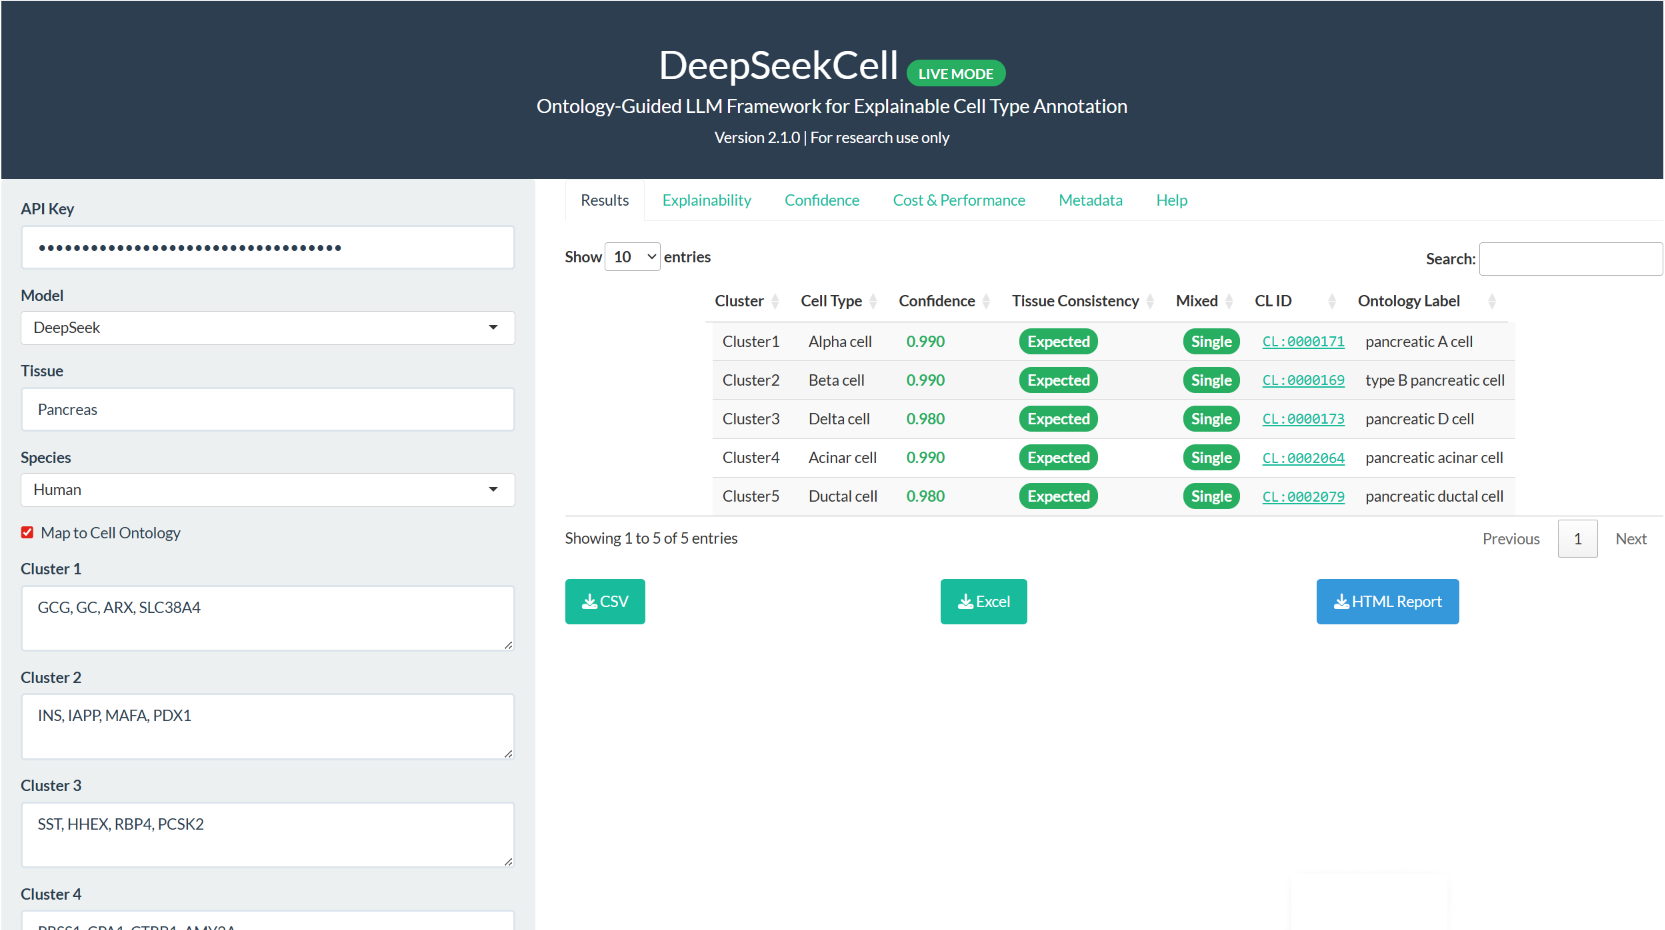
\includegraphics[width=\textwidth]{deepseekcell_shiny_interface.png}
\caption{DeepSeekCell Shiny interface for interactive cell type annotation. The application accepts cluster marker genes, displays predicted cell types with confidence scores and Cell Ontology identifiers, and provides explainability, validation, cost, metadata, and report export views.}\label{fig:shiny}
\end{figure}

\subsection{Benchmark datasets}

We evaluated DeepSeekCell using a closed-label, marker-guided benchmark. DeepSeekCell is intended as a marker-driven annotation framework for cluster marker lists rather than a raw expression matrix classifier; therefore, the benchmark was designed to evaluate annotation from cluster-level markers. Six curated datasets were included: PBMC, BaronPancreas, MuraroPancreas, TasicBrain, ZeiselBrain, and ZilionisLung. The datasets spanned human PBMC, human pancreas, mouse brain, and human lung. For each dataset, Seurat-based preprocessing and clustering were used to produce cluster-level marker genes \cite{hao2021seurat,seurat}. The benchmark used the top 25 marker genes per cluster, Seurat resolution 0.5, and 50 principal components. Three benchmark replicates were run with seeds 100, 200, and 300. Fixed datasets were deterministic across replicates, while the ZilionisLung dataset used seed-dependent cell subsampling. Dataset characteristics and preprocessing summaries are shown in Table~\ref{tab:datasets}.

\subsection{Evaluation metrics}

DeepSeekCell was compared with SingleR, ScType, scmap, and CellTypist on the same cluster structure. SingleR, ScType, and scmap predictions were converted to cluster-level labels by majority vote where needed. scmap was evaluated using scmapCell nearest-neighbor label transfer, followed by cluster-level majority voting. CellTypist was run in its native cell-level setting using tissue-aware pretrained models where available: an immune model for PBMC, an adult pancreatic islet model for pancreas, and the Human Lung Atlas model for lung. Native cell-level CellTypist metrics were retained separately, and cluster-level CellTypist labels were derived by majority vote only for the shared cluster-level comparison. CellTypist was evaluated on human datasets and skipped for the two mouse brain datasets because the benchmark used a human-only baseline configuration for CellTypist. A specific CellTypist model can be selected through the \texttt{CELLTYPIST\_MODEL} environment variable. Optional baselines are skipped with an explicit message if their R or Python dependencies are unavailable. Predicted and reference labels were harmonized through explicit tissue-aware label rules before metric calculation.

Annotation performance was evaluated using adjusted Rand index (ARI), macro-F1 score, exact cluster-level accuracy, balanced accuracy, ontology-aware clade accuracy, unknown-label rate, ontology coverage, runtime, and LLM token/cost metadata. Ontology-aware clade accuracy considers a prediction correct when the predicted and reference labels are ontologically related at an accepted lineage level, allowing biologically related predictions to be distinguished from unrelated errors. Exploratory statistical comparisons were performed using paired Wilcoxon signed-rank tests across dataset-replicate blocks, comparing DeepSeekCell with each baseline for each metric. Friedman tests were used as omnibus repeated-measures tests across complete method sets. These tests were interpreted cautiously because only three replicates were available and several datasets were deterministic across replicates.

\subsection{Ablation and selector-control design}

The ablation benchmark used one cached first-pass DeepSeek response per dataset and replicate. The raw response text, prompt metadata, and MD5 response hash were stored and reused across all DeepSeekCell ablation arms, preventing API stochasticity from being mistaken for algorithmic improvement. Four non-refinement arms isolate first-pass annotation and uncertainty effects: DeepSeek-Plain uses first-pass labels and raw confidence; DeepSeekCell-Evidence computes deterministic evidence fields without changing labels or confidence; DeepSeekCell-Calibrated replaces the displayed confidence with the evidence-adjusted score without changing labels; and DeepSeekCell-SelfRefined selectively refines only evidence-conflicted clusters.

To test whether the selector itself contributes beyond merely giving the LLM another opportunity to answer, three compute-matched second-pass controls were evaluated with the same per-dataset refinement budget $k$: Random-k refines $k$ randomly selected clusters, Confidence-k refines the $k$ clusters with lowest first-pass confidence, and Evidence-k refines the clusters selected by the deterministic evidence-conflict rule. FullRefined refines every cluster and serves as an approximate upper-bound control. Classification metrics were interpreted separately from uncertainty metrics because DeepSeek-Plain, DeepSeekCell-Evidence, and DeepSeekCell-Calibrated intentionally use identical labels.

\subsubsection{Mathematical definition of evaluation metrics}

Let a benchmark dataset contain $n$ evaluated clusters. For cluster $i$, let $y_i$ denote the harmonized reference label and $\hat{y}_i$ denote the harmonized predicted label. Let $\mathcal{L}$ be the set of evaluated cell type labels and let $\mathbb{I}(\cdot)$ be the indicator function. Exact cluster-level accuracy was defined as
\begin{equation}
\mathrm{Accuracy}=\frac{1}{n}\sum_{i=1}^{n}\mathbb{I}(\hat{y}_i=y_i).
\label{eq:accuracy}
\end{equation}

For each label $\ell \in \mathcal{L}$, precision and recall were calculated from true positives ($TP_\ell$), false positives ($FP_\ell$), and false negatives ($FN_\ell$):
\begin{equation}
P_\ell=\frac{TP_\ell}{TP_\ell+FP_\ell}, \qquad
R_\ell=\frac{TP_\ell}{TP_\ell+FN_\ell}.
\label{eq:precision-recall}
\end{equation}
The macro-F1 score was then computed as the unweighted mean of class-specific F1 scores:
\begin{equation}
\mathrm{MacroF1}=\frac{1}{|\mathcal{L}|}\sum_{\ell\in\mathcal{L}}
\frac{2P_\ell R_\ell}{P_\ell+R_\ell}.
\label{eq:macrof1}
\end{equation}
Balanced accuracy was computed as the unweighted mean recall:
\begin{equation}
\mathrm{BalancedAccuracy}=\frac{1}{|\mathcal{L}|}\sum_{\ell\in\mathcal{L}}R_\ell.
\label{eq:balancedaccuracy}
\end{equation}

The adjusted Rand index was calculated from the contingency table $n_{ab}$ between predicted groups $a$ and reference groups $b$:
\begin{equation}
\mathrm{ARI}=
\frac{
\sum_{ab}\binom{n_{ab}}{2}
-\frac{\sum_a\binom{n_{a\cdot}}{2}\sum_b\binom{n_{\cdot b}}{2}}{\binom{n}{2}}
}{
\frac{1}{2}\left[\sum_a\binom{n_{a\cdot}}{2}+\sum_b\binom{n_{\cdot b}}{2}\right]
-\frac{\sum_a\binom{n_{a\cdot}}{2}\sum_b\binom{n_{\cdot b}}{2}}{\binom{n}{2}}
}.
\label{eq:ari}
\end{equation}

To incorporate Cell Ontology structure, each harmonized label was mapped to an ontology term when possible. Let $\Omega(\hat{y}_i,y_i)=1$ if the predicted and reference labels are exact matches or if their mapped Cell Ontology terms are accepted ancestor/descendant lineage relatives, and $\Omega(\hat{y}_i,y_i)=0$ otherwise. Ontology-aware clade accuracy was defined as
\begin{equation}
\mathrm{CladeAccuracy}=\frac{1}{n}\sum_{i=1}^{n}\Omega(\hat{y}_i,y_i).
\label{eq:cladeaccuracy}
\end{equation}
The unknown-label rate was defined as
\begin{equation}
\mathrm{UnknownRate}=\frac{1}{n}\sum_{i=1}^{n}\mathbb{I}(\hat{y}_i=\mathrm{Unknown}).
\label{eq:unknownrate}
\end{equation}
For each metric $m$ summarized across $R$ benchmark replicates, the reported mean and 95\% confidence interval were
\begin{equation}
\bar{m}=\frac{1}{R}\sum_{r=1}^{R}m_r,\qquad
\mathrm{CI}_{95}=t_{0.975,R-1}\frac{s_m}{\sqrt{R}},
\label{eq:ci}
\end{equation}
where $s_m$ is the standard deviation across replicates. Confidence intervals are zero for deterministic datasets and nonzero for seed-dependent subsampling results.

For refinement analysis, initially wrong and initially correct labels were defined relative to the harmonized first-pass prediction. Conflict precision and conflict recall were
\begin{equation}
\mathrm{ConflictPrecision}=\frac{N_{\mathrm{flagged\ and\ initially\ wrong}}}{N_{\mathrm{flagged}}},\qquad
\mathrm{ConflictRecall}=\frac{N_{\mathrm{flagged\ and\ initially\ wrong}}}{N_{\mathrm{initially\ wrong}}}.
\label{eq:conflict-pr}
\end{equation}
The net correction rate and correction efficiency were defined as
\begin{equation}
\mathrm{NetCorrectionRate}=\frac{N_{\mathrm{wrong\to correct}}-N_{\mathrm{correct\to wrong}}}{N_{\mathrm{refined}}},\qquad
\mathrm{CorrectionEfficiency}=\frac{N_{\mathrm{wrong\to correct}}}{N_{\mathrm{refined}}}.
\label{eq:correction-efficiency}
\end{equation}
Recovery fraction was calculated relative to full refinement:
\begin{equation}
\mathrm{RecoveryFraction}=\frac{N_{\mathrm{wrong\to correct, selector}}}{N_{\mathrm{wrong\to correct, full}}}.
\label{eq:recovery-fraction}
\end{equation}
Bootstrap confidence intervals for refinement-efficiency metrics were estimated by resampling dataset-replicate blocks with replacement.

\begin{table}[htp]
\caption{Benchmark datasets and preprocessing summary. Values are taken from the final three-replicate benchmark manifest. ZilionisLung cluster counts varied across seed-dependent subsampling replicates.}\label{tab:datasets}
\begin{tabular}{@{}llllrrrr@{}}
\toprule
Dataset & Tissue & Species & Cells & Genes & Clusters & Mean purity & Min purity\\
\midrule
PBMC & PBMC & Human & 2,700 & 13,714 & 8 & 0.941 & 0.844\\
BaronPancreas & Pancreas & Human & 8,569 & 20,125 & 16 & 0.952 & 0.534\\
MuraroPancreas & Pancreas & Human & 2,122 & 19,059 & 11 & 0.954 & 0.892\\
TasicBrain & Brain & Mouse & 1,809 & 24,058 & 15 & 0.929 & 0.692\\
ZeiselBrain & Brain & Mouse & 3,005 & 20,006 & 16 & 0.773 & 0.504\\
ZilionisLung & Lung & Human & 5,000 & 41,861 & 16--18 & 0.910 & 0.406--0.660\\
\botrule
\end{tabular}
\end{table}

\section{Results}\label{sec:results}

\subsection{Overall annotation performance}

The final benchmark run used three replicates and completed all reported method-dataset combinations, resulting in 192 full result rows and 64 dataset-method summaries. DeepSeek ablation arms, ScType, SingleR, and scmap were evaluated on all six datasets; CellTypist was evaluated on the four human datasets and skipped for the two mouse brain datasets. Every reported dataset-method combination had three successful runs. All clusters were evaluated, and no benchmark cluster truth remained labeled as unknown after label curation. The benchmark manifest recorded Cell Ontology loading, methods, top marker count, Seurat settings, cache version, first-pass response hashes, and dataset quality summaries.

Across the six datasets, the first-pass DeepSeek annotation achieved a mean macro-F1 of 0.733, exact accuracy of 0.741, and ontology-aware clade accuracy of 0.883 (Table~\ref{tab:overall}; Figs.~\ref{fig:macroF1} and \ref{fig:accuracy}). DeepSeekCell-SelfRefined increased mean macro-F1 to 0.794 and exact accuracy to 0.783 while maintaining high clade accuracy (0.893). FullRefined achieved the highest mean macro-F1 (0.808) and accuracy (0.810), but required refinement of every cluster. These results show that the proposed evidence-guided selector captures much of the full-refinement gain while using a substantially smaller refinement budget.

\subsection{Aggregate benchmark performance}

\begin{table}[htp]
\caption{Overall benchmark performance. Runtime is reported in seconds. CellTypist was evaluated on the four human datasets; the other methods were evaluated on all six datasets. DeepSeekCell-SelfRefined is the proposed evidence-guided selective-refinement method.}\label{tab:overall}
\small
\begin{tabularx}{\textwidth}{@{}Xrrrrr@{}}
\toprule
Method & Datasets & Mean macro-F1 & Mean accuracy & Mean clade accuracy & Mean runtime\\
\midrule
DeepSeekCell-FullRefined & 6 & 0.808 & 0.810 & 0.862 & 16.11\\
DeepSeekCell-SelfRefined & 6 & 0.794 & 0.783 & 0.893 & 9.99\\
DeepSeek-Plain & 6 & 0.733 & 0.741 & 0.883 & 9.22\\
ScType & 6 & 0.749 & 0.773 & 0.778 & 0.71\\
SingleR & 6 & 0.466 & 0.479 & 0.757 & 26.90\\
scmap & 6 & 0.411 & 0.438 & 0.702 & 15.11\\
CellTypist & 4 & 0.558 & 0.612 & 0.656 & 1.68\\
\botrule
\end{tabularx}
\end{table}

\begin{figure}[htp]
\centering

\includegraphics[width=\textwidth]{benchmark_macroF1.pdf}
\caption{Macro-F1 performance across benchmark datasets and methods. Bars represent the mean across three benchmark replicates. Error bars represent 95\% confidence intervals when replicate variability is present. CellTypist was evaluated on human datasets only.}\label{fig:macroF1}
\end{figure}

\begin{figure}[htp]
\centering

\includegraphics[width=\textwidth]{benchmark_accuracy.pdf}
\caption{Exact cluster-level annotation accuracy across benchmark datasets. DeepSeekCell-SelfRefined improved accuracy relative to the first-pass LLM while using selective second-pass refinement.}\label{fig:accuracy}
\end{figure}

\subsection{Exploratory statistical analysis}

Paired Wilcoxon signed-rank tests were performed across dataset-replicate blocks using DeepSeekCell-SelfRefined as the reference method. For macro-F1, DeepSeekCell-SelfRefined exceeded the first-pass LLM descriptively (mean difference 0.061; BH-adjusted \(P=0.068\)) and significantly exceeded SingleR (BH-adjusted \(P=0.021\)) and scmap (BH-adjusted \(P=0.010\)), while the difference from ScType was not significant (BH-adjusted \(P=0.315\)). For exact accuracy, DeepSeekCell-SelfRefined exceeded the first-pass LLM descriptively (mean difference 0.043; BH-adjusted \(P=0.062\)) and significantly exceeded scmap (BH-adjusted \(P=0.019\)), while differences from SingleR and ScType did not remain significant after correction. Friedman tests across the refinement-control arms showed significant differences for macro-F1 (\(P=0.011\)), accuracy (\(P=0.009\)), clade accuracy (\(P=0.003\)), and runtime (\(P=8.14\times10^{-12}\)). Full test outputs are provided in Supplementary Tables S6 and S7.

\subsection{Evidence-guided confidence calibration}

Confidence quality was evaluated separately from classification accuracy because DeepSeek-Plain, DeepSeekCell-Evidence, and DeepSeekCell-Calibrated intentionally use the same labels. Replacing the raw LLM confidence with the evidence-adjusted confidence reduced the mean Brier score from 0.138 to 0.130 and reduced binary correctness negative log-likelihood from 0.441 to 0.422 while leaving labels unchanged. Expected calibration error changed only modestly (0.197 to 0.194), and AUROC decreased from 0.796 to 0.714, indicating that the evidence-adjusted score improved average probability alignment but did not uniformly improve ranking of correct versus incorrect predictions. After selective refinement, DeepSeekCell-SelfRefined obtained the lowest Brier score (0.125) and binary correctness negative log-likelihood (0.410) among the DeepSeekCell arms.

\subsection{Controlled selective-refinement benchmark}

The central methodological experiment tested whether deterministic biological evidence can identify the clusters that benefit most from a second LLM pass. FullRefined corrected 22 initially wrong labels after refining 249 clusters, corresponding to 8.8\% correction efficiency. In contrast, evidence-guided selective refinement corrected 13 initially wrong labels after refining only 16 clusters, corresponding to 81.3\% correction efficiency. Under the same refinement budget of 16 clusters, Random-k corrected 9 labels and Confidence-k corrected 7 labels (Table~\ref{tab:refinement-efficiency}; Fig.~\ref{fig:refinement-efficiency}).

Evidence-guided selective refinement recovered 59.1\% of all corrections achieved by full refinement while refining only 6.4\% as many clusters. Its bootstrap 95\% confidence interval for correction efficiency was 71.4--100.0\%, compared with 0.0--85.7\% for Random-k, 0.0--58.1\% for Confidence-k, and 0.0--20.8\% for FullRefined. No refinement strategy introduced incorrect revisions of previously correct annotations across the benchmark. Paired selector tests showed that Evidence-k significantly exceeded Confidence-k for wrong-to-correct revisions and net correction count after BH correction (both adjusted \(P=0.039\)). Evidence-k also exceeded Random-k descriptively, but this difference was not significant in the current dataset-replicate sample (adjusted \(P=0.330\) for wrong-to-correct revisions). These results indicate that the evidence-guided selector contributes beyond simply providing the LLM with an additional opportunity to answer.

\begin{table}[htp]
\caption{Controlled refinement-selector efficiency. Correction efficiency is wrong-to-correct revisions divided by the number of refined clusters. Recovery fraction is calculated relative to the wrong-to-correct revisions achieved by full refinement.}\label{tab:refinement-efficiency}
\begin{tabular}{@{}lrrrrr@{}}
\toprule
Selector & Refined & Wrong to correct & Correct to wrong & Efficiency & Recovery\\
\midrule
FullRefined & 249 & 22 & 0 & 8.8\% & 100.0\%\\
SelfRefined & 16 & 13 & 0 & 81.3\% & 59.1\%\\
Random-k & 16 & 9 & 0 & 56.3\% & 40.9\%\\
Confidence-k & 16 & 7 & 0 & 43.8\% & 31.8\%\\
\botrule
\end{tabular}
\end{table}

\begin{figure}[htp]
\centering
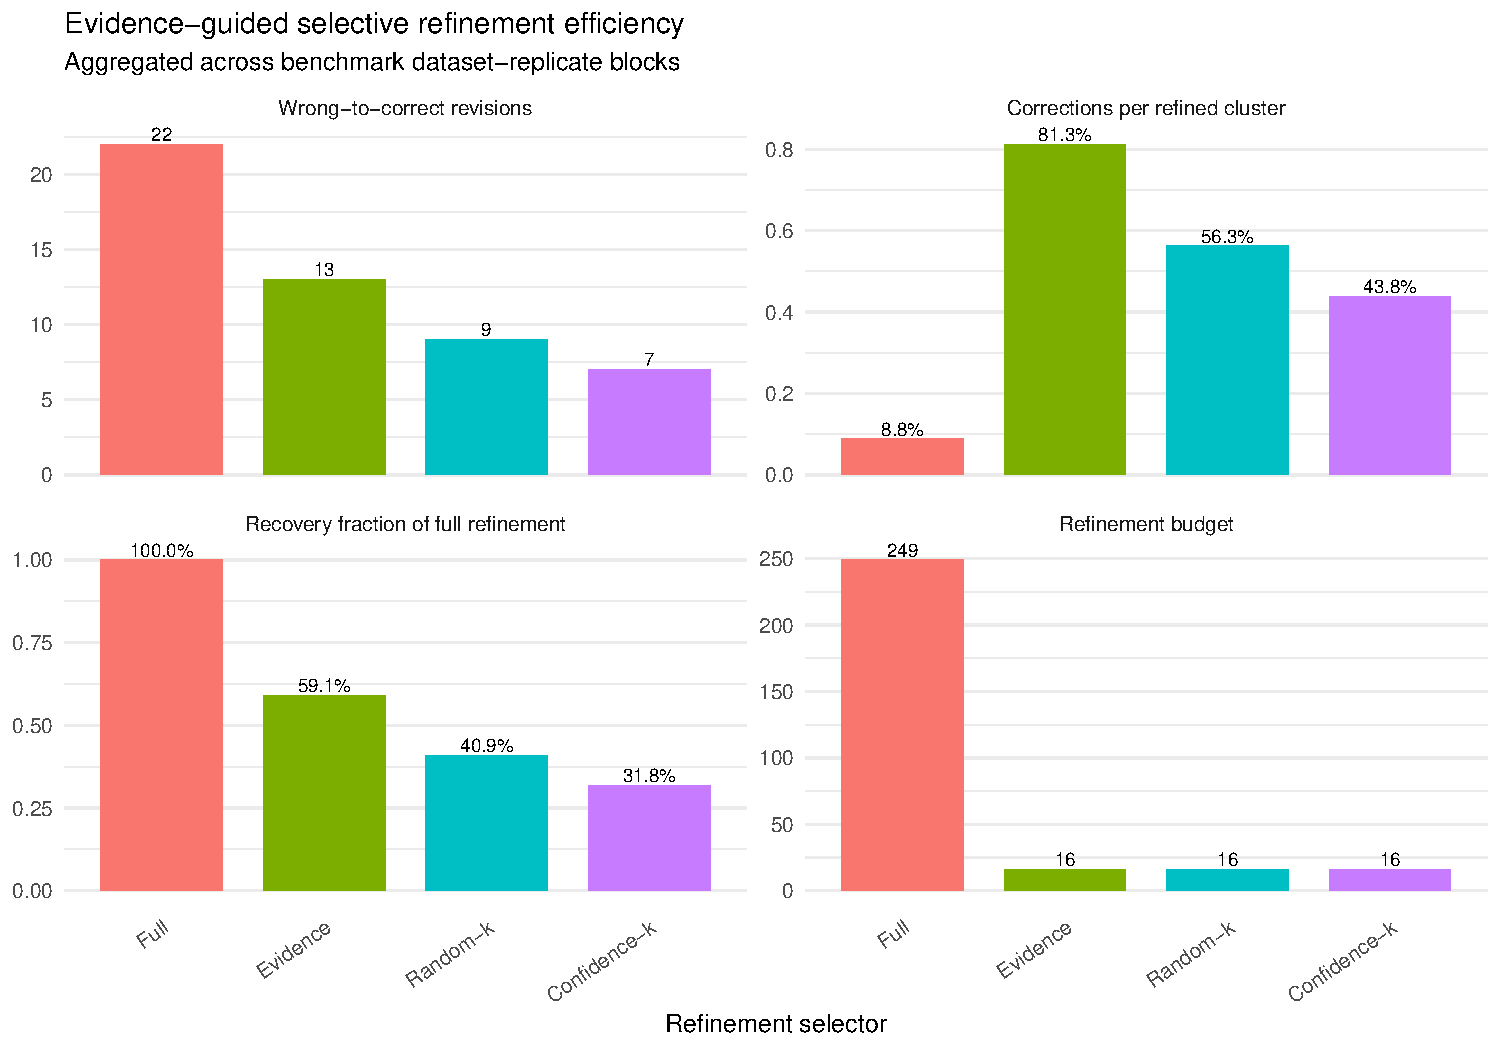
\includegraphics[width=\textwidth]{refinement_efficiency.pdf}
\caption{Evidence-guided selective refinement efficiency. Panels show wrong-to-correct revisions, correction efficiency, recovery fraction relative to full refinement, and refinement budget. Evidence-guided selection recovered most of the attainable full-refinement corrections while using a small fixed refinement budget.}\label{fig:refinement-efficiency}
\end{figure}

\subsection{Dataset-level benchmark performance}

In BaronPancreas, ScType achieved the highest macro-F1 (0.947), followed by DeepSeekCell-SelfRefined (0.852). In MuraroPancreas, ScType again had the highest macro-F1 (0.958), while DeepSeekCell-SelfRefined remained competitive (0.917). SingleR and scmap showed lower exact accuracy in both pancreas datasets but high ontology-aware clade accuracy, suggesting that some predictions were ontologically related even when exact labels differed. Native CellTypist performance was lower in the pancreas benchmarks despite use of a pancreatic islet model, reflecting cross-study label granularity and model-domain differences.

In TasicBrain, DeepSeekCell-SelfRefined achieved perfect macro-F1, exact accuracy, and clade accuracy. In ZeiselBrain, all methods showed lower macro-F1 compared with other datasets, consistent with the lower mean cluster purity of this dataset (0.773). DeepSeekCell-SelfRefined achieved the highest macro-F1 in ZeiselBrain (0.590), slightly above ScType (0.580) and SingleR (0.579), and improved over the first-pass LLM (0.465).

In ZilionisLung, SingleR achieved the highest macro-F1 (0.659), followed by FullRefined (0.613), scmap (0.531), CellTypist (0.524), DeepSeekCell-SelfRefined (0.407), Random-k (0.373), Confidence-k (0.325), and ScType (0.163). Although DeepSeekCell-SelfRefined did not surpass reference-based baselines in this dataset, it improved substantially over the first-pass LLM macro-F1 (0.166) using a limited selective-refinement budget. Confidence intervals were nonzero in ZilionisLung because cell subsampling varied across benchmark seeds, producing 16--18 clusters across replicates. Runtime comparisons are shown in Fig.~\ref{fig:runtime}. Dataset-level macro-F1 results are summarized in Table~\ref{tab:datasetlevel}.

\begin{table}[htp]
\caption{Dataset-level macro-F1 summary.}\label{tab:datasetlevel}
\small
\begin{tabularx}{\textwidth}{@{}llXrr@{}}
\toprule
Dataset & Tissue & Best method & Best macro-F1 & SelfRefined macro-F1\\
\midrule
PBMC & PBMC & DeepSeekCell-SelfRefined & 1.000 & 1.000\\
BaronPancreas & Pancreas & ScType & 0.947 & 0.852\\
MuraroPancreas & Pancreas & ScType & 0.958 & 0.917\\
TasicBrain & Brain & DeepSeekCell-SelfRefined & 1.000 & 1.000\\
ZeiselBrain & Brain & DeepSeekCell-SelfRefined & 0.590 & 0.590\\
ZilionisLung & Lung & SingleR & 0.659 & 0.407\\
\botrule
\end{tabularx}
\end{table}

\subsection{Explainability analysis}

DeepSeekCell outputs concise biological reasoning alongside each predicted label. For PBMC-like marker sets, expression of canonical T cell genes such as \textit{CD3D} and \textit{CD3E} supports T cell annotation and mapping to CL:0000084. For pancreatic endocrine marker sets, expression of \textit{INS} and \textit{IAPP} supports beta cell annotation and mapping to CL:0000169. These examples illustrate how DeepSeekCell connects marker evidence, cell type prediction, confidence, tissue consistency, and ontology identifiers in a single reviewable output.

\subsection{LLM reproducibility and stability}

The benchmark used a temperature of 0 for DeepSeek API calls to reduce stochastic variation. Per-cluster debug files were used to assess DeepSeekCell label stability across the five fixed cluster-structure datasets. Across PBMC, BaronPancreas, MuraroPancreas, TasicBrain, and ZeiselBrain, all 66 comparable clusters had identical raw and harmonized DeepSeekCell predictions across the three benchmark replicates, corresponding to an overall fixed-dataset stability rate of 1.000. The ZilionisLung dataset was excluded from this label-stability summary because seed-dependent subsampling changed the cluster structures across replicates. The manuscript-level stability summary is shown in Table~\ref{tab:stability}, and full stability summaries are provided in Supplementary Table S8.

\begin{table}[htp]
\caption{DeepSeekCell annotation stability across repeated benchmark runs. Stability was calculated as the proportion of comparable clusters with identical harmonized DeepSeekCell labels across three benchmark replicates. ZilionisLung was excluded because seed-dependent cell subsampling changed the cluster structure across replicates.}\label{tab:stability}
\begin{tabular}{@{}lrrr@{}}
\toprule
Dataset & Comparable clusters & Replicates & Stability (\%)\\
\midrule
PBMC & 8 & 3 & 100.0\\
BaronPancreas & 16 & 3 & 100.0\\
MuraroPancreas & 11 & 3 & 100.0\\
TasicBrain & 15 & 3 & 100.0\\
ZeiselBrain & 16 & 3 & 100.0\\
Overall fixed-dataset summary & 66 & 3 & 100.0\\
\botrule
\end{tabular}
\end{table}

\subsection{Native CellTypist baseline}

CellTypist was evaluated in its native cell-level workflow on the four human datasets. Cell-level macro-F1 was 0.801 for PBMC, 0.298 for BaronPancreas, 0.362 for MuraroPancreas, and 0.481 for ZilionisLung. For the shared cluster-level benchmark, cell-level CellTypist predictions were converted to cluster labels by majority vote, yielding cluster-level macro-F1 values of 1.000, 0.333, 0.375, and 0.524 for the same datasets. CellTypist was skipped for the two mouse brain datasets under the human-only baseline configuration. This native evaluation addresses CellTypist in its intended setting while retaining a secondary cluster-level comparison for consistency with the marker-based benchmark.

\subsection{Computational performance}

DeepSeek-Plain required a mean runtime of 9.22 seconds across the six datasets, while DeepSeekCell-SelfRefined required 9.99 seconds and FullRefined required 16.11 seconds. The selective strategy therefore preserved most of the full-refinement correction benefit while avoiding refinement of 233 of 249 clusters. Across all dataset-replicate blocks, SelfRefined used 6,180 refinement tokens and 13.82 seconds of refinement runtime, compared with 75,385 refinement tokens and 124.13 seconds for FullRefined. The corresponding estimated refinement costs were USD 0.00110 for SelfRefined and USD 0.01353 for FullRefined. Thus, evidence-guided refinement recovered 59.1\% of the attainable corrections using 8.2\% of the full-refinement token budget and 11.1\% of the full-refinement runtime. ScType and native CellTypist were the fastest evaluated baselines on average (0.71 and 1.68 seconds, respectively), while SingleR and scmap required longer runtime in several reference-based comparisons. Runtime, token usage, estimated API cost, second-pass call count, and refinement budget are recorded for every LLM interaction. Runtime comparisons are shown in Fig.~\ref{fig:runtime}.

\subsection{Interactive Shiny platform}

The Shiny platform successfully loaded the Cell Ontology and displayed structured annotations containing predicted labels, confidence scores, tissue-consistency tags, mixed-cluster tags, Cell Ontology identifiers, ontology labels, match methods, and match scores. The explainability tab provided marker-based reasoning for each prediction, supporting review of why a label was assigned. Export functions generated CSV, Excel, and HTML outputs suitable for downstream reporting (Fig.~\ref{fig:shiny}). The detailed dataset-level benchmark values supporting the summary comparisons are reported in Table~\ref{tab:detailed}.

\begin{table}[htp]
\caption{Detailed dataset-level benchmark performance. Values are means across three benchmark replicates. CI values are omitted here for compactness and are available in \texttt{final\_benchmark\_table.csv}.}\label{tab:detailed}
\scriptsize
\begin{tabularx}{\textwidth}{@{}lXrrrrr@{}}
\toprule
Dataset & Method & Macro-F1 & Accuracy & Clade acc. & Unknown & Runtime\\
\midrule
BaronPancreas & ScType & 0.947 & 0.938 & 0.923 & 0.000 & 0.80\\
BaronPancreas & DeepSeekCell-SelfRefined & 0.852 & 0.771 & 0.846 & 0.000 & 11.46\\
BaronPancreas & SingleR & 0.222 & 0.125 & 1.000 & 0.000 & 123.57\\
BaronPancreas & scmap & 0.222 & 0.125 & 1.000 & 0.000 & 49.38\\
BaronPancreas & CellTypist & 0.333 & 0.438 & 0.462 & 0.000 & 1.44\\
MuraroPancreas & ScType & 0.958 & 0.909 & 0.889 & 0.000 & 0.54\\
MuraroPancreas & DeepSeekCell-SelfRefined & 0.917 & 0.818 & 0.875 & 0.091 & 8.05\\
MuraroPancreas & CellTypist & 0.375 & 0.545 & 0.556 & 0.000 & 0.86\\
MuraroPancreas & SingleR & 0.125 & 0.091 & 0.750 & 0.000 & 12.61\\
MuraroPancreas & scmap & 0.125 & 0.091 & 0.750 & 0.000 & 4.87\\
PBMC & CellTypist & 1.000 & 1.000 & 1.000 & 0.000 & 1.45\\
PBMC & DeepSeekCell-SelfRefined & 1.000 & 1.000 & 1.000 & 0.000 & 5.45\\
PBMC & ScType & 0.875 & 0.875 & 0.875 & 0.000 & 1.51\\
PBMC & SingleR & 0.542 & 0.625 & 0.714 & 0.000 & 3.14\\
PBMC & scmap & 0.396 & 0.500 & 0.548 & 0.000 & 6.18\\
TasicBrain & DeepSeekCell-SelfRefined & 1.000 & 1.000 & 1.000 & 0.000 & 9.17\\
TasicBrain & ScType & 0.971 & 0.933 & 0.933 & 0.000 & 0.35\\
TasicBrain & SingleR & 0.667 & 0.600 & 0.643 & 0.067 & 4.03\\
TasicBrain & scmap & 0.633 & 0.600 & 0.600 & 0.000 & 4.07\\
ZeiselBrain & DeepSeekCell-SelfRefined & 0.590 & 0.750 & 0.867 & 0.063 & 10.99\\
ZeiselBrain & ScType & 0.580 & 0.750 & 0.813 & 0.000 & 0.45\\
ZeiselBrain & SingleR & 0.579 & 0.750 & 0.750 & 0.000 & 5.75\\
ZeiselBrain & scmap & 0.558 & 0.688 & 0.688 & 0.000 & 6.96\\
ZilionisLung & SingleR & 0.659 & 0.684 & 0.684 & 0.000 & 12.31\\
ZilionisLung & CellTypist & 0.524 & 0.466 & 0.607 & 0.000 & 2.96\\
ZilionisLung & scmap & 0.531 & 0.625 & 0.625 & 0.000 & 19.22\\
ZilionisLung & DeepSeekCell-SelfRefined & 0.407 & 0.360 & 0.770 & 0.480 & 14.80\\
ZilionisLung & ScType & 0.163 & 0.235 & 0.235 & 0.000 & 0.62\\
\botrule
\end{tabularx}
\end{table}

\begin{figure}[htp]
\centering

\includegraphics[width=\textwidth]{benchmark_clade_accuracy.pdf}
\caption{Cell Ontology-aware clade accuracy across benchmark datasets. This metric credits predictions that are ontologically related to the reference label, capturing biologically meaningful agreement beyond exact string matching.}\label{fig:cladeacc}
\end{figure}

\begin{figure}[htp]
\centering

\includegraphics[width=\textwidth]{benchmark_runtime.pdf}
\caption{Runtime comparison across evaluated methods. DeepSeekCell-SelfRefined adds selective second-pass reasoning to the first-pass LLM, while FullRefined invokes a second pass for every cluster. ScType and CellTypist were fast baselines, and SingleR and scmap showed longer runtimes in larger reference-based comparisons.}\label{fig:runtime}
\end{figure}

\section{Discussion}\label{sec:discussion}

DeepSeekCell demonstrates that LLM-based cell type annotation can be improved by treating second-pass reasoning as a limited resource. The main contribution is not simply the use of DeepSeek for marker interpretation, but an evidence-guided selector that combines deterministic marker, ontology, and tissue-consistency signals to identify clusters where additional reasoning is most likely to correct an error. This reframes LLM annotation from a single prompting task into a cost-aware refinement problem. Because the selector operates on structured annotation outputs and deterministic biological evidence, it is not specific to DeepSeek and could be paired with other instruction-following LLMs.

The fixed-budget selector experiment directly addresses an alternative explanation: that improvement arises merely because the LLM is asked a second time. Random-k, Confidence-k, and Evidence-k received the same refinement budget, but the evidence-guided selector corrected more initially wrong labels than either control and introduced no correct-to-wrong revisions. Evidence-guided selective refinement recovered 59.1\% of the full-refinement corrections while refining only 6.4\% as many clusters. This result suggests that deterministic biological evidence can guide efficient allocation of expensive or rate-limited LLM inference.

The benchmark should be interpreted as a marker-driven cluster annotation benchmark rather than a raw expression matrix benchmark. This design matches the intended DeepSeekCell input representation and the common manual workflow in which analysts inspect top cluster markers before assigning identities. In this setting, DeepSeekCell-SelfRefined was strongest when marker genes clearly encoded canonical cell identities, such as immune populations in PBMC and neuronal/glial classes in TasicBrain. In pancreas datasets, ScType remained strongest, likely reflecting strong marker database coverage for pancreatic endocrine and exocrine cell types. In ZilionisLung, SingleR performed best by macro-F1, while DeepSeekCell-SelfRefined improved over the first-pass LLM and retained high ontology-aware clade accuracy, suggesting that ontology-level evaluation can capture biologically related predictions missed by exact string matching.

The ZeiselBrain dataset highlights an important limitation: benchmark accuracy depends on cluster purity and label granularity. Lower mean cluster purity can make cluster-level annotation ambiguous for all methods. DeepSeekCell therefore reports tissue consistency, mixed-cluster flags, confidence, and ontology match metadata to help users identify annotations requiring manual review.

This study has several limitations. First, the benchmark is cluster-level and marker-guided for DeepSeekCell, and therefore evaluates annotation from marker evidence rather than direct classification from raw or normalized expression matrices. Second, although CellTypist was evaluated in its native cell-level workflow, its cluster-level results required majority-vote aggregation and were limited to human datasets under the selected pretrained models. Third, the evidence weights were prespecified heuristic weights rather than learned calibration coefficients; future studies should evaluate sensitivity analyses and held-out calibration. Fourth, ontology evidence is partly label-dependent: a wrong but valid label can still map well to the Cell Ontology, so ontology support should be interpreted as semantic and nomenclatural support rather than proof of biological correctness. Fifth, marker profiles are manually curated and finite, so unsupported or poorly characterized cell states may receive conservative evidence scores. Sixth, the statistical analyses are exploratory because only three replicates were run and most datasets were deterministic across replicates; only the ZilionisLung dataset included seed-dependent subsampling variability. Seventh, stability was assessed at the label-output level for fixed benchmark cluster structures, but additional work is needed to test stability across model versions, prompt revisions, and larger repeated LLM call sets. Finally, LLM-generated reasoning should be treated as an explanatory aid rather than independent biological proof.

Future work will extend the method in three directions. First, evidence weights should be evaluated through sensitivity analysis, held-out calibration, or simple fitted calibration models such as logistic regression or isotonic regression. Second, the selector should be tested across more tissues, disease states, perturbation datasets, and additional LLM backends to determine whether refinement efficiency generalizes beyond DeepSeek. Third, the Shiny platform will be expanded to support automatic marker extraction from Seurat objects, file upload for arbitrary marker tables, larger cluster counts, multi-modal annotation, expanded ontology integration, and optional offline annotation modes.

\section{Conclusions}\label{sec:conclusions}

DeepSeekCell introduces evidence-guided selective refinement for marker-based LLM annotation of scRNA-seq clusters. By combining structured first-pass annotation, Cell Ontology mapping, deterministic marker and tissue evidence, evidence-adjusted confidence, and selective second-pass reasoning, the framework identifies a small subset of clusters where additional LLM inference is most useful. The benchmark shows that this selector recovers most attainable full-refinement corrections at a fraction of the refinement budget, supporting DeepSeekCell as a methods framework for explainable and cost-aware single-cell annotation.

\section*{List of abbreviations}

ARI: adjusted Rand index; AURC: area under the risk-coverage curve; BMC: BioMed Central; CL: Cell Ontology identifier; ECE: expected calibration error; LLM: large language model; NLL: negative log-likelihood; PBMC: peripheral blood mononuclear cell; PCA: principal component analysis; scRNA-seq: single-cell RNA sequencing.

\backmatter

\bmhead{Supplementary information}

Supplementary table captions are provided for the CSV files included with the submission package. Supplementary Table S1: full replicate-level benchmark results from \texttt{benchmark\_results\_full.csv}, including ARI, macro-F1, exact accuracy, balanced accuracy, clade accuracy, unknown rate, runtime, token usage, estimated cost, cluster purity, and refinement metadata. Supplementary Table S2: benchmark summary statistics from \texttt{benchmark\_results\_summary.csv}. Supplementary Table S3: dataset-level preprocessing and cluster purity summaries from \texttt{dataset\_summary.csv}. Supplementary Table S4: cluster-level truth labels and cluster purity summaries from \texttt{cluster\_summary.csv}. Supplementary Table S5: compact final benchmark table from \texttt{final\_benchmark\_table.csv}. Supplementary Table S6: paired Wilcoxon signed-rank comparisons from \texttt{benchmark\_pairwise\_wilcoxon.csv}. Supplementary Table S7: Friedman omnibus tests from \texttt{benchmark\_friedman\_tests.csv}. Supplementary Table S8: DeepSeekCell label stability summaries from \texttt{benchmark\_llm\_stability.csv}. Supplementary Table S9: confidence-quality metrics from \texttt{ablation\_confidence\_quality.csv}. Supplementary Table S10: reliability-bin summaries from \texttt{ablation\_reliability\_bins.csv}. Supplementary Table S11: refinement-behaviour outputs from \texttt{ablation\_refinement\_behavior.csv}. Supplementary Table S12: aggregate refinement-efficiency summary from \texttt{refinement\_efficiency\_summary.csv}. Supplementary Table S13: paired selector-comparison tests from \texttt{refinement\_selector\_pairwise\_wilcoxon.csv}. Supplementary Table S14: native cell-level CellTypist metrics from \texttt{celltypist\_native\_cell\_metrics.csv}. Supplementary global benchmark overview plots are provided for ARI (Fig.~\ref{fig:supp-global-ari}), macro-F1 (Fig.~\ref{fig:supp-global-macroF1}), exact accuracy (Fig.~\ref{fig:supp-global-accuracy}), and runtime (Fig.~\ref{fig:supp-global-runtime}).

\begin{figure}[htp]
\centering
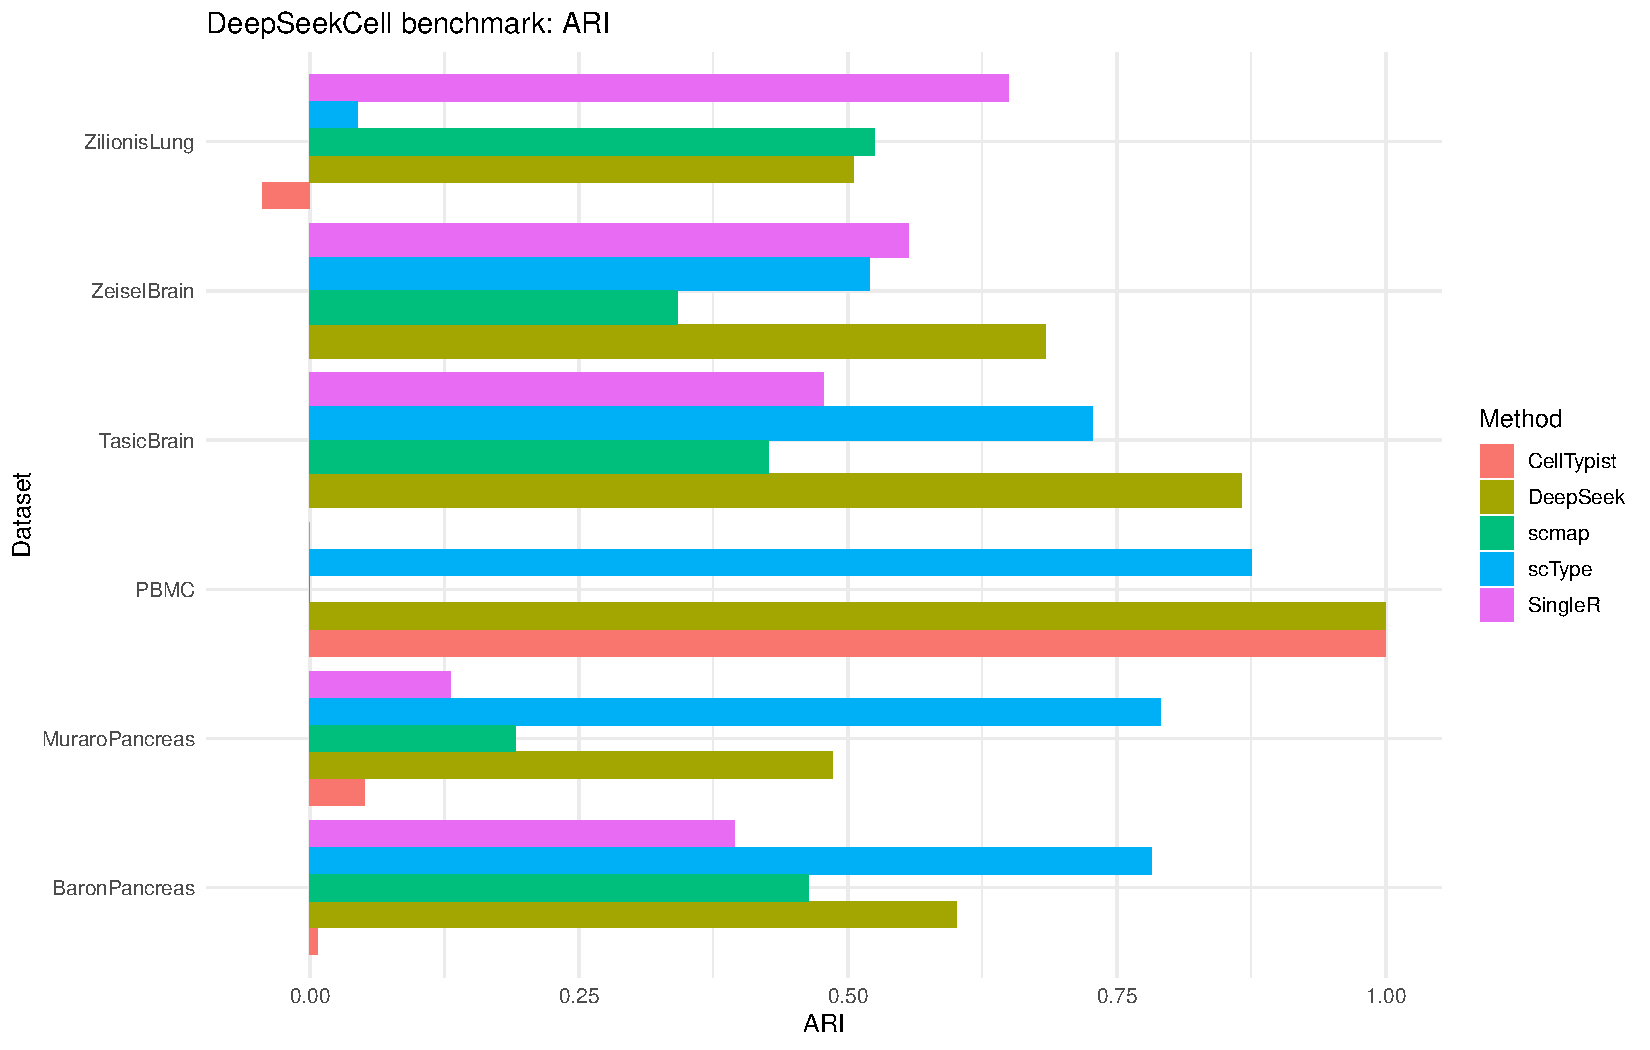
\includegraphics[width=\textwidth]{global_ARI.pdf}
\caption{Supplementary global benchmark overview for adjusted Rand index (ARI). Bars summarize mean ARI by dataset and method.}\label{fig:supp-global-ari}
\end{figure}

\begin{figure}[htp]
\centering
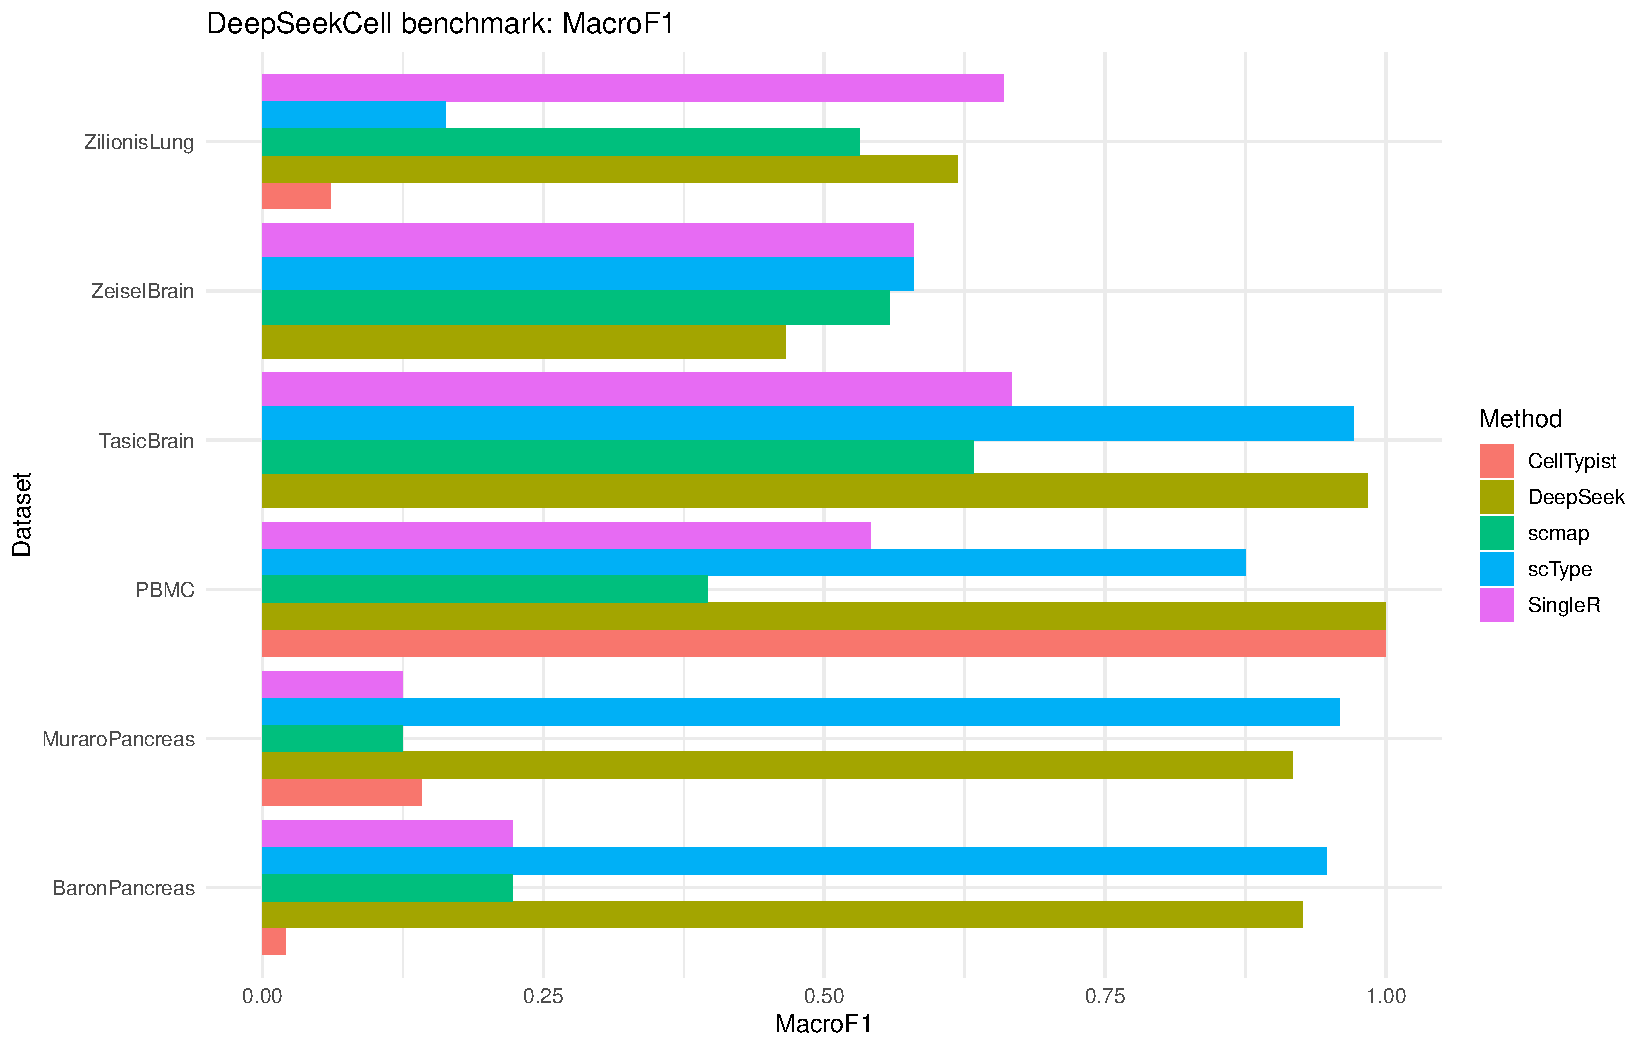
\includegraphics[width=\textwidth]{global_MacroF1.pdf}
\caption{Supplementary global benchmark overview for macro-F1. Bars summarize mean macro-F1 by dataset and method.}\label{fig:supp-global-macroF1}
\end{figure}

\begin{figure}[htp]
\centering
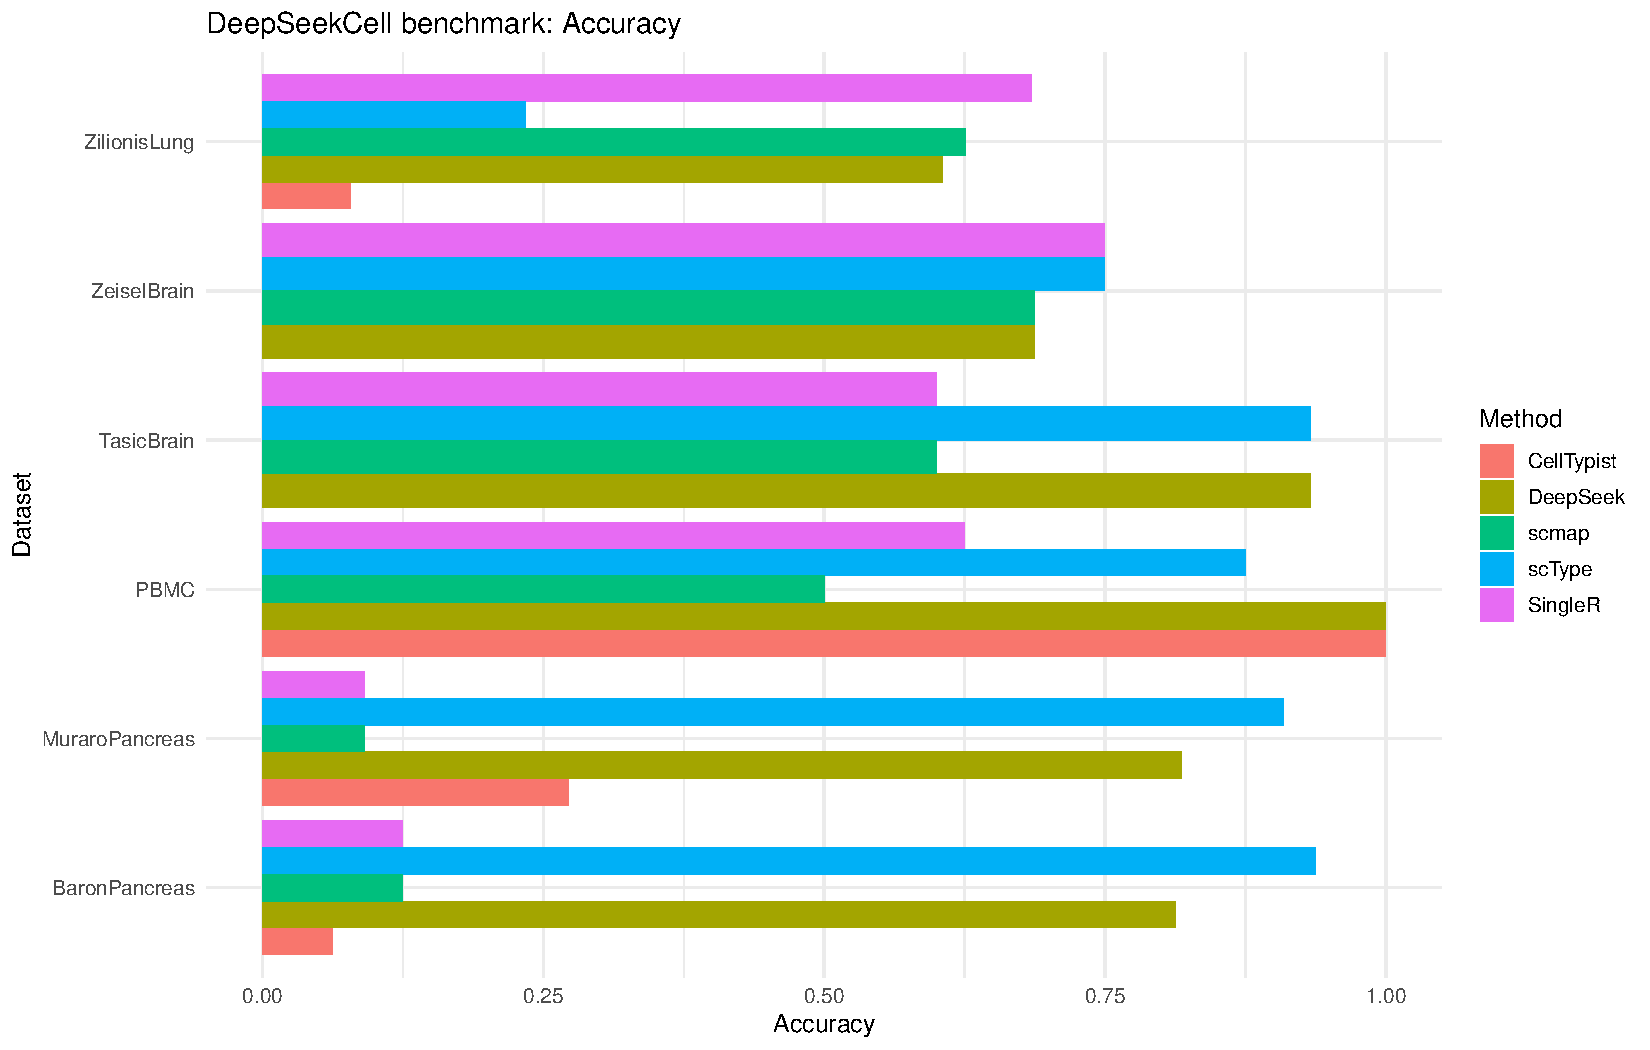
\includegraphics[width=\textwidth]{global_Accuracy.pdf}
\caption{Supplementary global benchmark overview for exact annotation accuracy. Bars summarize mean exact accuracy by dataset and method.}\label{fig:supp-global-accuracy}
\end{figure}

\begin{figure}[htp]
\centering
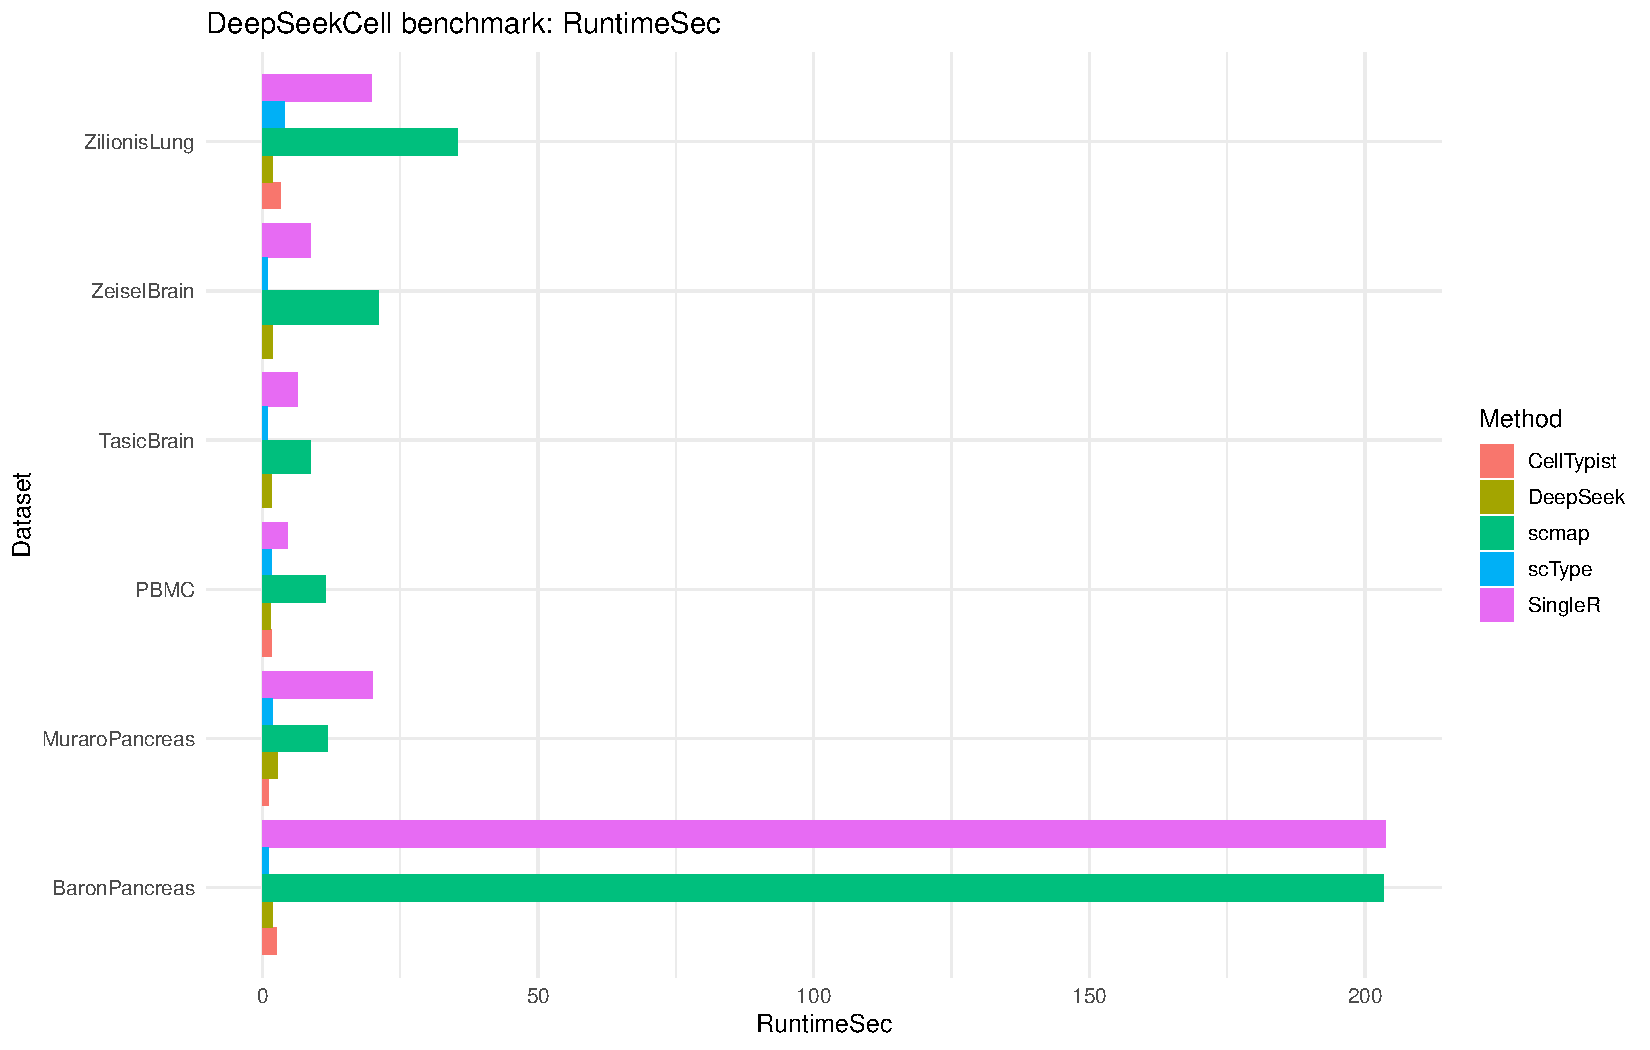
\includegraphics[width=\textwidth]{global_Runtime.pdf}
\caption{Supplementary global benchmark overview for runtime. Bars summarize mean runtime by dataset and method.}\label{fig:supp-global-runtime}
\end{figure}

\section*{Declarations}

\bmhead{Ethics approval and consent to participate}
Not applicable. This study used public or package-distributed benchmark datasets and did not involve new human participant recruitment, new animal experiments, or new collection of human samples.

\bmhead{Consent for publication}
Not applicable.

\bmhead{Availability of data and materials}
The source code is available at \url{https://github.com/mohkone/DeepSeekCell.git}. The archived GitHub-Zenodo software record is available at \url{https://doi.org/10.5281/zenodo.20680434}, with all-version concept DOI \url{https://doi.org/10.5281/zenodo.20680433}. Benchmark scripts are provided in the \texttt{benchmarks/} directory. The final benchmark outputs used for this manuscript are generated locally in the \texttt{results/} directory, including \texttt{final\_benchmark\_table.csv}, \texttt{benchmark\_results\_full.csv}, \texttt{benchmark\_results\_summary.csv}, \texttt{dataset\_summary.csv}, \texttt{cluster\_summary.csv}, \texttt{benchmark\_pairwise\_wilcoxon.csv}, \texttt{benchmark\_friedman\_tests.csv}, \texttt{benchmark\_llm\_stability.csv}, \texttt{ablation\_confidence\_quality.csv}, \texttt{ablation\_reliability\_bins.csv}, \texttt{ablation\_refinement\_behavior.csv}, \texttt{refinement\_efficiency\_summary.csv}, \texttt{refinement\_selector\_pairwise\_wilcoxon.csv}, \texttt{celltypist\_native\_cell\_metrics.csv}, and \texttt{benchmark\_manifest.txt}. Large external resources, including the full Cell Ontology OBO file and ScType database, should be obtained according to their upstream licenses.

\bmhead{Competing interests}
The authors declare that they have no competing interests.

\bmhead{Funding}
The authors received no specific funding for this work.

\bmhead{Code availability}
Project name: DeepSeekCell. Project home page: \url{https://github.com/mohkone/DeepSeekCell.git}. Archived software record: \url{https://doi.org/10.5281/zenodo.20680434}; all-version concept DOI: \url{https://doi.org/10.5281/zenodo.20680433}. Manuscript software version: DeepSeekCell 0.1.0, corresponding to benchmark cache version \texttt{2026-06-12-publication-v5}. Operating system: platform independent. Programming language: R. Other requirements: R 4.1 or later and the R package dependencies listed in the repository \texttt{DESCRIPTION} file. License: MIT. Restrictions for non-academic use: none beyond the software license and the licenses of external resources used by the workflow.

\bmhead{Authors' contributions}
M.K., S.W., and G.H. conceived the study, developed the DeepSeekCell software and Shiny platform, designed and interpreted the benchmark analyses, and wrote and revised the manuscript. All authors reviewed and approved the final manuscript.

\bmhead{Acknowledgements}
The authors thank the developers and maintainers of the open-source R, Shiny, Seurat, SingleR, ScType, and Cell Ontology resources used by this project.

\bmhead{Authors' information}
Not applicable.

\bibliographystyle{plain}
\bibliography{deepseekcell_bmc_refs}

\end{document}
